\chapter{Metodología}
\label{chap:metodologia}

\section{Diagnóstico de la Situación Actual}
Antes de diseñar una solución es necesario describir cómo se gestiona hoy la información que esta debe organizar. En el caso del proyecto Kallarimanta, el conocimiento sobre el patrimonio cultural inmaterial Kichwa de la Sierra Sur se encuentra distribuido en investigaciones académicas, archivos audiovisuales, documentos institucionales, registros comunitarios y testimonios orales, tal como se expuso en el planteamiento del problema. Estos recursos no están integrados en un sistema común, por lo que su localización, actualización y relación entre sí dependen del conocimiento personal de quienes los produjeron.

La investigación reciente del propio Centro de Investigación de Ciencias Humanas y de la Educación (CICHE) confirma que este conocimiento se genera de manera continua y que su gestión exige cuidados especiales. Quezada-Sarmiento \textit{et al.} \cite{quezada2026culinary} documentaron el patrimonio culinario de Saraguro mediante grupos focales con doce portadores de conocimiento, discusiones apoyadas en preparaciones tradicionales y actividades colaborativas con cocineros y estudiantes. En ese estudio, los autores declaran que los materiales cualitativos obtenidos están vinculados con conocimientos y protocolos culturales de la comunidad y que, por ese motivo, no se publican de forma abierta por defecto \cite{quezada2026culinary}. Esta declaración muestra que el proyecto ya produce información que no puede tratarse como un conjunto de datos público, sino que requiere un repositorio con control de acceso, registro del consentimiento y criterios de publicación definidos con la comunidad.

En el plano tecnológico, el antecedente directo es el prototipo móvil desarrollado para el patrimonio Saraguro \cite{quezada2026mobile}. Se trata de una aplicación para Android construida con el patrón MVVM y servicios de Firebase, cuyos propios autores señalan cuatro limitaciones: no permite la consulta sin conexión, ofrece un soporte multilingüe reducido, no se evaluó con un protocolo estandarizado de usabilidad y carece de un módulo de administración y validación comunitaria de los contenidos \cite{quezada2026mobile}. En la práctica, esto significa que incorporar una nueva manifestación exige la intervención del equipo técnico y que no existe un mecanismo explícito para que la comunidad apruebe lo que se publica sobre ella.

A escala nacional, el Instituto Nacional de Patrimonio Cultural administra el Sistema de Información del Patrimonio Cultural Ecuatoriano (SIPCE) y publica datos abiertos sobre las fichas de inventario del patrimonio inmaterial \cite{inpc2026sipce,inpc2025datos}. Sin embargo, como se analizó en el estado del arte, estas herramientas tienen un propósito administrativo y de alcance nacional, y no ofrecen funciones educativas, uso móvil sin conexión ni niveles de reserva definidos por cada comunidad.

La Tabla~\ref{tab:diagnostico} sintetiza las limitaciones técnicas identificadas y el requerimiento que cada una origina. Este diagnóstico es preliminar y se completará con los resultados de las entrevistas y grupos focales descritos en la sección de técnicas de recolección de información, que corresponden al objetivo específico~1.

\needspace{20\baselineskip}
{\centering\singlespacing
  \captionof{table}{Limitaciones de la situación actual y requerimientos que originan.}
  \label{tab:diagnostico}
  \begin{tabular}{|p{0.30\textwidth}|p{0.30\textwidth}|p{0.28\textwidth}|}
    \hline
    \textbf{Limitación actual} & \textbf{Consecuencia} & \textbf{Requerimiento derivado} \tabularnewline
    \hline
    \raggedright\hspace{0pt}Información dispersa en múltiples formatos y fuentes sin normalizar & \raggedright\hspace{0pt}Dificultad para localizar, actualizar y relacionar los registros & \raggedright\hspace{0pt}Repositorio central con fichas estructuradas y metadatos \tabularnewline
    \hline
    \raggedright\hspace{0pt}Ausencia de un módulo de administración en el prototipo existente & \raggedright\hspace{0pt}La carga de contenidos depende del equipo técnico & \raggedright\hspace{0pt}Aplicación web administrativa \tabularnewline
    \hline
    \raggedright\hspace{0pt}Ausencia de validación comunitaria y de niveles de acceso & \raggedright\hspace{0pt}Riesgo de publicar conocimiento reservado o sagrado & \raggedright\hspace{0pt}Flujo de validación, niveles de acceso y registro del consentimiento \tabularnewline
    \hline
    \raggedright\hspace{0pt}Ubicaciones registradas sin distinguir lugares sensibles & \raggedright\hspace{0pt}Posible exposición de sitios ceremoniales & \raggedright\hspace{0pt}Georreferenciación con ubicación aproximada para lugares sensibles \tabularnewline
    \hline
    \raggedright\hspace{0pt}Conectividad limitada en sectores rurales & \raggedright\hspace{0pt}Imposibilidad de consultar los contenidos sin Internet & \raggedright\hspace{0pt}Aplicación móvil con consulta sin conexión \tabularnewline
    \hline
    \raggedright\hspace{0pt}Soporte multilingüe reducido & \raggedright\hspace{0pt}Contenidos disponibles casi solo en español & \raggedright\hspace{0pt}Contenidos en español y kichwa con traducción validada \tabularnewline
    \hline
    \raggedright\hspace{0pt}Falta de un protocolo estandarizado de evaluación & \raggedright\hspace{0pt}No es posible comparar la calidad de uso entre versiones & \raggedright\hspace{0pt}Evaluación de usabilidad con la escala SUS \tabularnewline
    \hline
  \end{tabular}\par}
\elaboradopor{Michael Jhosue Almeida Díaz}
\fuente{Elaboración propia a partir de \cite{quezada2026mobile,quezada2026culinary}}

\section{Área de Estudio}

\begin{table}[htbp]
  \centering
  \caption{Área de estudio.}
  \label{tab:area_estudio}
  \renewcommand{\arraystretch}{1.35}
  \begin{tabular}{|p{0.39\textwidth}|p{0.53\textwidth}|}
    \hline
    \textbf{Dominio:} & Tecnologías de la información aplicadas al patrimonio cultural y a la educación intercultural. \\
    \hline
    \textbf{Línea de investigación:} & \UTILineaInvestigacion \\
    \hline
    \textbf{Sublínea de investigación:} & \UTISublineaInvestigacion \\
    \hline
    \textbf{Campo:} & Tecnologías de la información y la comunicación (TIC) \\
    \hline
    \textbf{Área:} & Ingeniería de software: desarrollo de aplicaciones web y móviles multiplataforma con componentes geoespaciales. \\
    \hline
    \textbf{Aspectos:} & Requerimientos, arquitectura de software, modelo de datos espacial, desarrollo web y móvil, funcionamiento sin conexión, control de acceso, validación comunitaria y usabilidad. \\
    \hline
    \textbf{Objeto de estudio:} & Gestión, georreferenciación y difusión educativa del patrimonio cultural inmaterial Kichwa documentado por el proyecto Kallarimanta (CICHE, Universidad Tecnológica Indoamérica), con comunidades piloto de Saraguro, Paltas y Cañar. \\
    \hline
    \textbf{Periodo de estudio:} & Año 2026 [PENDIENTE: fechas de inicio y fin del periodo académico]. \\
    \hline
  \end{tabular}
\end{table}

\section{Metodología de Desarrollo o Implementación}
Como se explicó en la fundamentación teórica, el trabajo combina dos niveles metodológicos. En el nivel de la investigación, Design Science Research (DSR) orienta el proceso completo, desde la identificación del problema hasta la evaluación y la comunicación del artefacto \cite{peffers2007dsrm}. En el nivel de la construcción del software, se utiliza Scrum como marco de gestión del producto \cite{schwaber2020scrum}, complementado con Mobile-D para organizar las actividades técnicas propias de la aplicación móvil \cite{abrahamsson2004mobiled}. La Imagen~\ref{img:integracion_metodologia} muestra cómo se articulan los tres niveles.

\begin{imagen}[htbp]
  \centering
  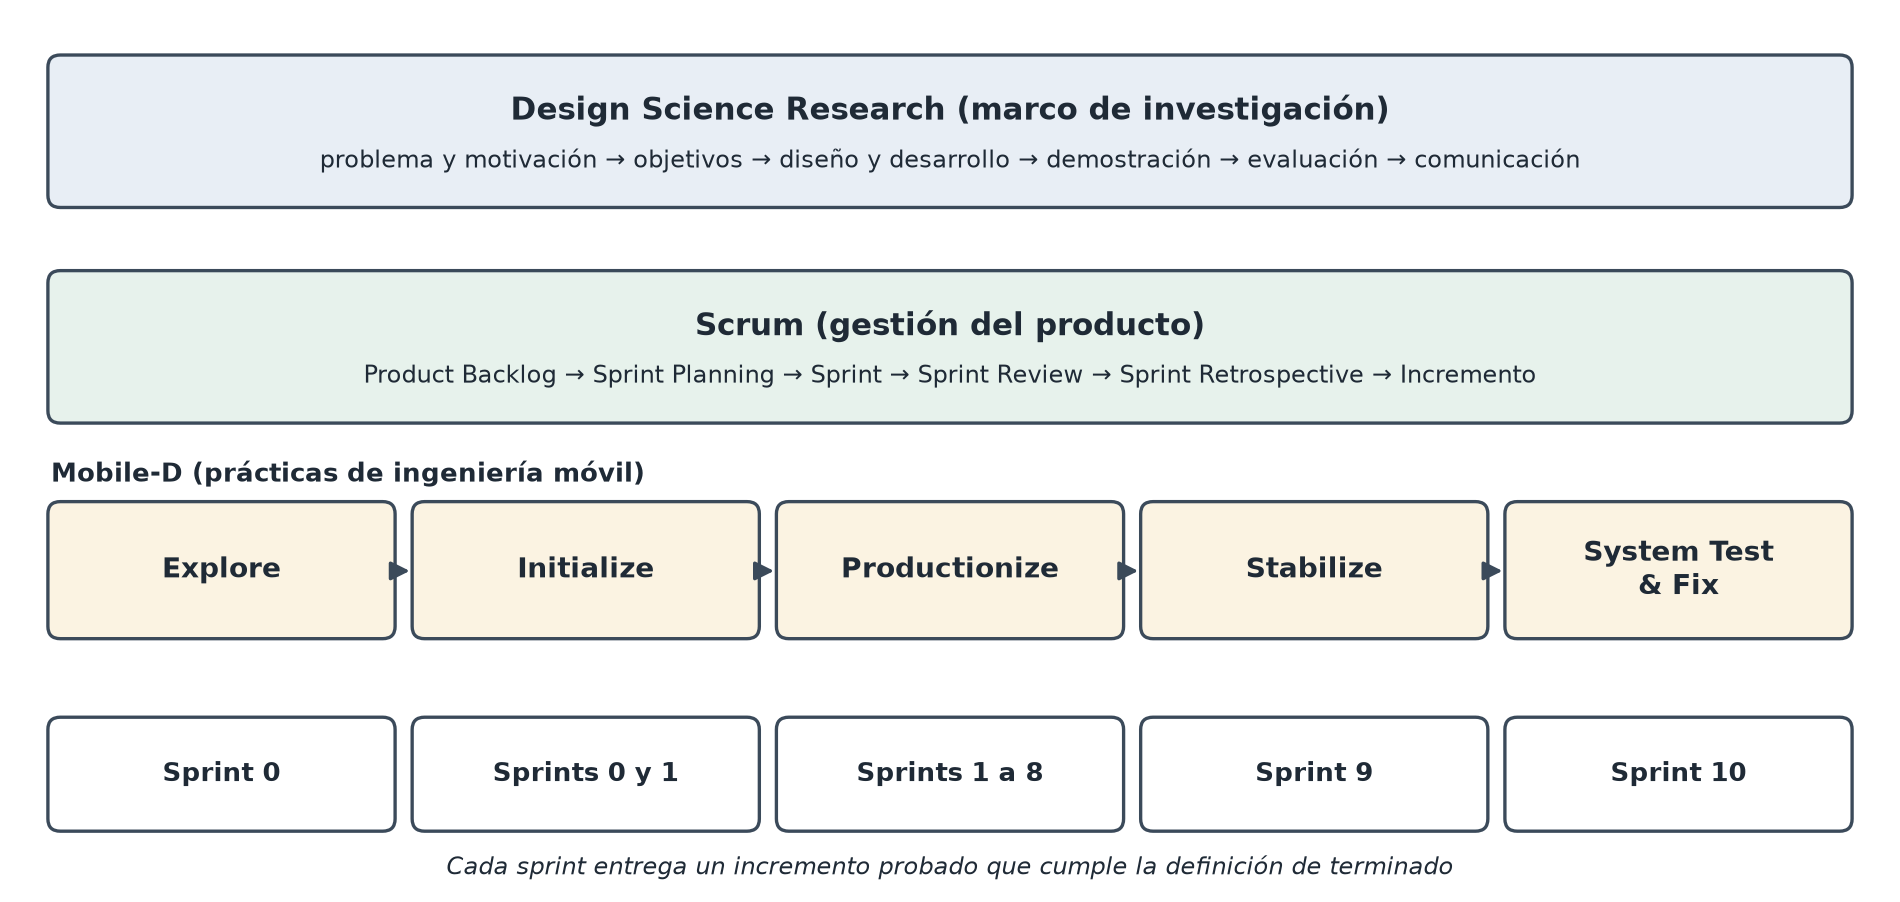
\includegraphics[width=0.95\textwidth]{Capítulos/img/integracion_metodologia.png}
  \caption{Integración de Design Science Research, Scrum y Mobile-D en el proyecto.}
  \label{img:integracion_metodologia}
\end{imagen}
\elaboradopor{Michael Jhosue Almeida Díaz}
\fuente{Elaboración propia a partir de \cite{peffers2007dsrm,schwaber2020scrum,abrahamsson2004mobiled}}

\subsection{Mobile-D como complemento de Scrum}
Mobile-D es una metodología ágil propuesta por Abrahamsson \textit{et al.} \cite{abrahamsson2004mobiled} para el desarrollo de aplicaciones móviles por equipos pequeños y en ciclos de entrega cortos. Una metodología \textit{ágil} es aquella que, en lugar de planificar todo el producto al inicio, lo construye en iteraciones breves y ajusta el plan según la retroalimentación obtenida. Mobile-D organiza el trabajo en cinco fases: \textit{Explore} (exploración), \textit{Initialize} (inicialización), \textit{Productionize} (producción), \textit{Stabilize} (estabilización) y \textit{System Test \& Fix} (prueba del sistema y corrección) \cite{abrahamsson2004mobiled}. Esta misma metodología fue la utilizada en el prototipo Saraguro que sirve de antecedente al presente trabajo \cite{quezada2026mobile}, lo que da continuidad técnica entre ambos desarrollos. La Tabla~\ref{tab:fases_mobiled} describe la aplicación de cada fase en este proyecto.

\needspace{12\baselineskip}
{\centering\singlespacing
  \captionof{table}{Fases de Mobile-D aplicadas al proyecto.}
  \label{tab:fases_mobiled}
  \begin{tabular}{|p{0.21\textwidth}|p{0.52\textwidth}|p{0.15\textwidth}|}
    \hline
    \textbf{Fase} & \textbf{Aplicación al proyecto} & \textbf{Sprints} \tabularnewline
    \hline
    \raggedright\hspace{0pt}\textit{Explore} & \raggedright\hspace{0pt}Definir alcance, usuarios, escenarios de uso, dispositivos y restricciones de conectividad & \raggedright\hspace{0pt}Sprint 0 \tabularnewline
    \hline
    \raggedright\hspace{0pt}\textit{Initialize} & \raggedright\hspace{0pt}Preparar repositorio, entornos e integración continua; definir arquitectura, modelo de datos y prototipos & \raggedright\hspace{0pt}Sprints 0 y 1 \tabularnewline
    \hline
    \raggedright\hspace{0pt}\textit{Productionize} & \raggedright\hspace{0pt}Construir las funcionalidades por incrementos, con pruebas e integración continuas & \raggedright\hspace{0pt}Sprints 1 a 8 \tabularnewline
    \hline
    \raggedright\hspace{0pt}\textit{Stabilize} & \raggedright\hspace{0pt}Integrar módulos, corregir defectos y verificar sincronización, rendimiento y permisos & \raggedright\hspace{0pt}Sprint 9 \tabularnewline
    \hline
    \raggedright\hspace{0pt}\textit{System Test \& Fix} & \raggedright\hspace{0pt}Pruebas de sistema, aceptación, seguridad y compatibilidad; correcciones finales & \raggedright\hspace{0pt}Sprint 10 \tabularnewline
    \hline
  \end{tabular}\par}
\elaboradopor{Michael Jhosue Almeida Díaz}
\fuente{Elaboración propia a partir de \cite{abrahamsson2004mobiled}}

Scrum y Mobile-D no se excluyen, sino que responden a preguntas distintas. Scrum define \textit{cómo se gestiona} el producto: qué se prioriza, cómo se planifica cada iteración y cómo se revisan los resultados. Mobile-D, en cambio, define \textit{qué actividades técnicas} requiere un producto móvil en cada etapa, como definir los dispositivos y escenarios de uso, preparar el entorno, construir las funcionalidades, integrarlas y probar el sistema completo. Por ello, en este proyecto se conservan los eventos y artefactos de Scrum y se utilizan las fases de Mobile-D como guía de las tareas técnicas que se incluyen en cada sprint. La relación entre ambas es funcional y no una equivalencia rígida entre fase y sprint.

\subsection{Roles y participación de los actores}
La Tabla~\ref{tab:roles_scrum} muestra cómo se asignan las responsabilidades de Scrum en un proyecto desarrollado por un solo estudiante, según la adaptación descrita en la fundamentación teórica. Conviene subrayar que la validación cultural no es una responsabilidad formal de Scrum. Por ello, la participación de los representantes comunitarios se incorpora de tres maneras: como interesados en las revisiones de los sprints, como fuente de criterios de aceptación de las historias de usuario y como validadores dentro del flujo editorial de la propia plataforma.

\needspace{16\baselineskip}
{\centering\singlespacing
  \captionof{table}{Responsabilidades de Scrum adaptadas al proyecto.}
  \label{tab:roles_scrum}
  \begin{tabular}{|p{0.20\textwidth}|p{0.32\textwidth}|p{0.36\textwidth}|}
    \hline
    \textbf{Rol} & \textbf{Definición en Scrum} & \textbf{Aplicación al proyecto} \tabularnewline
    \hline
    \raggedright\hspace{0pt}Dueño del producto & \raggedright\hspace{0pt}Maximizar el valor del producto y ordenar la lista de producto & \raggedright\hspace{0pt}Proyecto Kallarimanta, representado por el tutor y los investigadores del CICHE \tabularnewline
    \hline
    \raggedright\hspace{0pt}Scrum Master & \raggedright\hspace{0pt}Velar por la aplicación de Scrum y eliminar obstáculos & \raggedright\hspace{0pt}Estudiante, con la orientación del tutor \tabularnewline
    \hline
    \raggedright\hspace{0pt}Desarrollador & \raggedright\hspace{0pt}Construir en cada sprint un incremento utilizable & \raggedright\hspace{0pt}Estudiante: backend, web, móvil, datos y pruebas \tabularnewline
    \hline
    \raggedright\hspace{0pt}Interesados & \raggedright\hspace{0pt}Revisar los incrementos y aportar retroalimentación & \raggedright\hspace{0pt}Representantes comunitarios, docentes y estudiantes \tabularnewline
    \hline
  \end{tabular}\par}
\elaboradopor{Michael Jhosue Almeida Díaz}
\fuente{Elaboración propia a partir de \cite{schwaber2020scrum}}

\subsection{Planificación de los sprints}
El trabajo se organiza en once sprints de dos semanas cada uno como referencia de planificación, de modo que el desarrollo completo abarca aproximadamente veintidós semanas. La duración podrá ajustarse en las retrospectivas si la carga de trabajo real lo requiere. Las Tablas~\ref{tab:plan_sprints} y~\ref{tab:plan_sprints2} presentan el objetivo de cada sprint, los requerimientos funcionales que aborda, el objetivo específico al que contribuye y su criterio de salida, es decir, la condición que debe cumplirse para darlo por cerrado.

\needspace{30\baselineskip}
{\centering\singlespacing
  \captionof{table}{Planificación de los sprints del proyecto.}
  \label{tab:plan_sprints}
  \begin{tabular}{|p{0.07\textwidth}|p{0.30\textwidth}|p{0.13\textwidth}|p{0.08\textwidth}|p{0.24\textwidth}|}
    \hline
    \textbf{Sprint} & \textbf{Objetivo y entregables} & \textbf{RF} & \textbf{OE} & \textbf{Criterio de salida} \tabularnewline
    \hline
    \raggedright\hspace{0pt}0 & \raggedright\hspace{0pt}Requerimientos, historias de usuario, prototipos y arquitectura & \raggedright\hspace{0pt}--- & \raggedright\hspace{0pt}OE1, OE2 & \raggedright\hspace{0pt}Lista de producto priorizada y arquitectura aprobada \tabularnewline
    \hline
    \raggedright\hspace{0pt}1 & \raggedright\hspace{0pt}Autenticación, usuarios y roles; contenedores e integración continua & \raggedright\hspace{0pt}RF-01, RF-02, RF-17 & \raggedright\hspace{0pt}OE3 & \raggedright\hspace{0pt}Inicio de sesión y permisos por rol probados \tabularnewline
    \hline
    \raggedright\hspace{0pt}2 & \raggedright\hspace{0pt}Comunidades y categorías culturales & \raggedright\hspace{0pt}RF-03, RF-04 & \raggedright\hspace{0pt}OE3 & \raggedright\hspace{0pt}Catálogos gestionables desde la web \tabularnewline
    \hline
    \raggedright\hspace{0pt}3 & \raggedright\hspace{0pt}Manifestaciones, traducciones y multimedia con consentimiento & \raggedright\hspace{0pt}RF-05, RF-07, RF-14, RF-16 & \raggedright\hspace{0pt}OE3 & \raggedright\hspace{0pt}Ficha completa con recursos y consentimiento \tabularnewline
    \hline
    \raggedright\hspace{0pt}4 & \raggedright\hspace{0pt}Georreferenciación y mapas web & \raggedright\hspace{0pt}RF-06 & \raggedright\hspace{0pt}OE5 & \raggedright\hspace{0pt}Registro y consulta geográfica con lugares sensibles protegidos \tabularnewline
    \hline
    \raggedright\hspace{0pt}5 & \raggedright\hspace{0pt}Búsqueda, validación y publicación & \raggedright\hspace{0pt}RF-08, RF-09 & \raggedright\hspace{0pt}OE3 & \raggedright\hspace{0pt}Flujo editorial completo y auditado \tabularnewline
    \hline
      \end{tabular}\par}
\elaboradopor{Michael Jhosue Almeida Díaz}
\fuente{Elaboración propia}

\needspace{22\baselineskip}
{\centering\singlespacing
  \captionof{table}{Planificación de los sprints del proyecto (continuación).}
  \label{tab:plan_sprints2}
  \begin{tabular}{|p{0.07\textwidth}|p{0.30\textwidth}|p{0.13\textwidth}|p{0.08\textwidth}|p{0.24\textwidth}|}
    \hline
    \textbf{Sprint} & \textbf{Objetivo y entregables} & \textbf{RF} & \textbf{OE} & \textbf{Criterio de salida} \tabularnewline
    \hline
    \raggedright\hspace{0pt}6 & \raggedright\hspace{0pt}Aplicación móvil: consulta y mapa & \raggedright\hspace{0pt}RF-10, RF-11 & \raggedright\hspace{0pt}OE4, OE5 & \raggedright\hspace{0pt}Consulta y mapa funcionales en Android \tabularnewline
    \hline
    \raggedright\hspace{0pt}7 & \raggedright\hspace{0pt}Aplicación móvil sin conexión y sincronización & \raggedright\hspace{0pt}RF-12 & \raggedright\hspace{0pt}OE4 & \raggedright\hspace{0pt}Consulta demostrable sin Internet \tabularnewline
    \hline
    \raggedright\hspace{0pt}8 & \raggedright\hspace{0pt}Recursos educativos y reportes & \raggedright\hspace{0pt}RF-13, RF-15 & \raggedright\hspace{0pt}OE3, OE4 & \raggedright\hspace{0pt}Fichas y cuestionarios utilizables en la aplicación \tabularnewline
    \hline
    \raggedright\hspace{0pt}9 & \raggedright\hspace{0pt}Integración, pruebas, carga de contenidos y evaluación SUS & \raggedright\hspace{0pt}--- & \raggedright\hspace{0pt}Todos & \raggedright\hspace{0pt}Pruebas de usabilidad y regresión aprobadas \tabularnewline
    \hline
    \raggedright\hspace{0pt}10 & \raggedright\hspace{0pt}Correcciones finales, despliegue y documentación & \raggedright\hspace{0pt}--- & \raggedright\hspace{0pt}Todos & \raggedright\hspace{0pt}Versión candidata que cumple la definición de terminado \tabularnewline
    \hline
  \end{tabular}\par}
\elaboradopor{Michael Jhosue Almeida Díaz}
\fuente{Elaboración propia}

\subsection{Artefactos y definición de terminado}
La lista de producto (\textit{Product Backlog}) se redacta en forma de historias de usuario. Una \textit{historia de usuario} es una descripción breve de una funcionalidad escrita desde el punto de vista de quien la necesita, normalmente con la forma ``como [rol], quiero [acción] para [beneficio]'' \cite{cohn2004user}. Esta forma de redacción obliga a explicitar quién se beneficia de cada funcionalidad y por qué, lo que facilita su priorización por parte del dueño del producto. Cada historia se acompaña de criterios de aceptación, que son las condiciones verificables que debe cumplir para considerarse terminada. Las historias principales se presentan en la sección de requerimientos.

Para todo el proyecto se adopta la siguiente definición de terminado. Una funcionalidad se considera terminada cuando:

\begin{itemize}
  \item cumple los criterios de aceptación de su historia de usuario;
  \item su código está integrado en la rama principal del repositorio y supera la integración continua;
  \item cuenta con pruebas unitarias o de integración que se ejecutan sin errores;
  \item no presenta defectos críticos ni altos abiertos;
  \item respeta las reglas de control de acceso y registra las acciones auditables cuando corresponde;
  \item está documentada en la especificación OpenAPI de la API, si expone un servicio; y
  \item puede demostrarse en la revisión del sprint en el entorno de pruebas.
\end{itemize}

\section{Técnicas e Instrumentos de Recolección de Información}
Una \textit{técnica} de recolección de información es el procedimiento que se utiliza para obtener los datos, mientras que el \textit{instrumento} es el recurso concreto con el que se registran, por ejemplo, una guía de preguntas o un cuestionario. El proyecto requiere información en dos momentos: durante el diagnóstico y el levantamiento de requerimientos, que corresponden a la actividad de definición de objetivos de la DSR, y durante la validación del prototipo, que corresponde a la evaluación. La Tabla~\ref{tab:tecnicas} resume las técnicas empleadas.

\needspace{26\baselineskip}
{\centering\singlespacing
  \captionof{table}{Técnicas e instrumentos de recolección de información.}
  \label{tab:tecnicas}
  \begin{tabular}{|p{0.16\textwidth}|p{0.19\textwidth}|p{0.20\textwidth}|p{0.20\textwidth}|p{0.07\textwidth}|}
    \hline
    \textbf{Técnica} & \textbf{Instrumento} & \textbf{Participantes o fuentes} & \textbf{Propósito} & \textbf{OE} \tabularnewline
    \hline
    \raggedright\hspace{0pt}Revisión documental & \raggedright\hspace{0pt}Matriz de revisión documental & \raggedright\hspace{0pt}Materiales del proyecto Kallarimanta, prototipo Saraguro y datos del INPC & \raggedright\hspace{0pt}Identificar categorías, campos y contenidos existentes & \raggedright\hspace{0pt}OE1 \tabularnewline
    \hline
    \raggedright\hspace{0pt}Entrevista semiestructurada & \raggedright\hspace{0pt}Guía de entrevista & \raggedright\hspace{0pt}Docentes e investigadores del CICHE & \raggedright\hspace{0pt}Levantar requerimientos funcionales y educativos & \raggedright\hspace{0pt}OE1 \tabularnewline
    \hline
    \raggedright\hspace{0pt}Grupo focal & \raggedright\hspace{0pt}Protocolo de discusión semiestructurado & \raggedright\hspace{0pt}Representantes comunitarios y portadores de saberes & \raggedright\hspace{0pt}Definir niveles de acceso, lugares sensibles y requisitos lingüísticos & \raggedright\hspace{0pt}OE1 \tabularnewline
    \hline
    \raggedright\hspace{0pt}Validación de prototipos & \raggedright\hspace{0pt}Prototipos navegables y lista de observaciones & \raggedright\hspace{0pt}Usuarios representativos de cada rol & \raggedright\hspace{0pt}Validar requerimientos e interfaces antes de programar & \raggedright\hspace{0pt}OE2 \tabularnewline
    \hline
    \raggedright\hspace{0pt}Pruebas de software & \raggedright\hspace{0pt}Casos de prueba, colecciones de la API y reportes automáticos & \raggedright\hspace{0pt}Prototipo funcional & \raggedright\hspace{0pt}Verificar requerimientos funcionales y no funcionales & \raggedright\hspace{0pt}OE3 a OE5 \tabularnewline
    \hline
    \raggedright\hspace{0pt}Prueba de usabilidad & \raggedright\hspace{0pt}Guion de tareas, ficha de observación y cuestionario SUS & \raggedright\hspace{0pt}Estudiantes, docentes, investigadores y representantes comunitarios & \raggedright\hspace{0pt}Evaluar efectividad, eficiencia y satisfacción & \raggedright\hspace{0pt}OE4 \tabularnewline
    \hline
  \end{tabular}\par}
\elaboradopor{Michael Jhosue Almeida Díaz}
\fuente{Elaboración propia}

\subsection{Revisión documental}
La revisión documental consiste en analizar de forma sistemática los documentos existentes para extraer la información relevante. En este proyecto se revisarán los materiales recopilados por el proyecto Kallarimanta, la estructura de contenidos del prototipo Saraguro \cite{quezada2026mobile} y el diccionario de datos de las fichas de inventario del patrimonio inmaterial publicadas por el INPC \cite{inpc2025datos}. El instrumento es una matriz que registra, para cada fuente, el tipo de información que contiene, los campos que utiliza y su utilidad para el modelo de datos. Su principal resultado será la lista inicial de categorías culturales y de campos de la ficha patrimonial.

\subsection{Entrevista semiestructurada}
La entrevista semiestructurada es una conversación guiada por un conjunto de preguntas preparadas de antemano, pero que permite al entrevistador formular nuevas preguntas según las respuestas obtenidas. Se aplicará a docentes e investigadores del CICHE vinculados con el proyecto Kallarimanta, con el fin de conocer cómo registran actualmente la información, qué tareas deben realizar en la plataforma y qué recursos educativos necesitan. La guía de entrevista se organizará en tres bloques: proceso actual de registro, funcionalidades esperadas y uso educativo de los contenidos.

\subsection{Grupo focal}
El grupo focal es una técnica cualitativa en la que un pequeño grupo de personas discute un tema guiado por un moderador, de modo que la información surge de la interacción entre los participantes y no solo de sus respuestas individuales \cite{hamui2013grupos}. Esta característica la hace adecuada para explorar significados compartidos y acuerdos colectivos, como los que se requieren para definir qué conocimientos pueden publicarse y cuáles deben reservarse.

La elección de esta técnica cuenta con un precedente directo en el mismo contexto. En el estudio sobre el patrimonio culinario de Saraguro, Quezada-Sarmiento \textit{et al.} \cite{quezada2026culinary} aplicaron un grupo focal con doce portadores de conocimiento seleccionados de forma intencional, moderado mediante un protocolo semiestructurado, y analizaron las transcripciones mediante análisis temático de contenido. En el presente proyecto, el grupo focal se realizará con representantes comunitarios y portadores de saberes, y su protocolo abordará tres temas: los criterios para clasificar un contenido como público, restringido o reservado; los lugares que deben mostrarse con ubicación aproximada; y las condiciones para la traducción y validación de los textos en kichwa.

\subsection{Validación de prototipos}
Un \textit{prototipo} es una versión preliminar de la interfaz que permite a los usuarios ver y probar cómo funcionará el sistema antes de que se programe. Sommerville \cite{sommerville2016software} señala que la construcción de prototipos es una técnica útil para validar los requerimientos, porque permite detectar malentendidos y necesidades no expresadas antes de que corregirlos resulte costoso. Durante el sprint~0 se elaborarán prototipos de las pantallas principales en Figma, que se revisarán con usuarios representativos de cada rol. Las observaciones se registrarán en una lista y se incorporarán a la lista de producto.

\subsection{Pruebas de software}
Las pruebas de software verifican que el sistema cumple sus requerimientos. Se aplicarán pruebas unitarias, que comprueban de forma aislada las reglas de negocio, por ejemplo, que un estudiante no pueda ver un contenido reservado; pruebas de integración, que comprueban el funcionamiento conjunto de la API y la base de datos; pruebas funcionales, mediante una lista de verificación por requerimiento; y pruebas de seguridad, compatibilidad y rendimiento. Los instrumentos serán los casos de prueba, las colecciones de solicitudes a la API y los reportes generados automáticamente por las herramientas de prueba.

\subsection{Prueba de usabilidad}
La prueba de usabilidad consiste en pedir a usuarios reales que realicen tareas concretas con el sistema mientras se observa su desempeño. Cada participante realizará un guion de tareas representativas de su rol, como buscar una manifestación, reproducir un audio, consultar un contenido sin conexión o validar una ficha. El observador registrará en una ficha si la tarea se completó, el tiempo empleado y los errores cometidos, lo que permite valorar la efectividad y la eficiencia definidas en la norma ISO 9241-11 \cite{iso2018usability}. Al finalizar, cada participante responderá el cuestionario SUS, cuya puntuación se calcula mediante la Ecuación~\ref{eq:sus} \cite{brooke1996sus}:

\begin{equation}
\label{eq:sus}
SUS = 2{,}5 \times \left[ \sum_{i \in \{1,3,5,7,9\}} (r_i - 1) + \sum_{i \in \{2,4,6,8,10\}} (5 - r_i) \right]
\end{equation}
\addeqtolist{Puntuación de la escala de usabilidad SUS}

\noindent donde $r_i$ es la respuesta del participante al ítem $i$, en una escala de 1 a 5. El resultado es un valor entre 0 y 100, y se adopta como referencia mínima el valor de 68, que corresponde al promedio de los sistemas evaluados con esta escala \cite{sauro2011sus}.

\subsection{Selección de participantes y consideraciones éticas}
Se utilizará un muestreo no probabilístico intencional, es decir, los participantes se seleccionarán por su conocimiento y su relación con el proyecto, y no al azar. Este criterio es el mismo que se aplicó en el estudio de referencia de Saraguro, donde se priorizó la experiencia cultural de los participantes sobre la representatividad estadística \cite{quezada2026culinary}. Por tanto, los resultados se interpretarán de forma descriptiva y no se generalizarán a toda la población. El número de participantes por grupo se definirá con el CICHE [PENDIENTE: número de participantes por técnica].

Todos los participantes firmarán un consentimiento informado que explique el propósito del estudio, el uso que se dará a la información y su derecho a retirarse. Los datos personales se tratarán conforme a la Ley Orgánica de Protección de Datos Personales del Ecuador \cite{ecuador2021lopdp}. Además, siguiendo el precedente del proyecto, los materiales que contengan conocimientos sujetos a protocolos culturales no se publicarán de forma abierta y su difusión requerirá la autorización de la comunidad \cite{quezada2026culinary,unesco2015ethical}.

\section{Requerimientos del Proyecto}
Según Sommerville \cite{sommerville2016software}, los requerimientos de un sistema son las descripciones de los servicios que debe prestar y de las restricciones bajo las cuales debe funcionar. Se distinguen dos tipos. Los \textit{requerimientos funcionales} describen lo que el sistema debe hacer, por ejemplo, registrar una manifestación o mostrar un mapa. Los \textit{requerimientos no funcionales} describen cómo debe hacerlo o qué cualidades debe tener, por ejemplo, su seguridad, su rendimiento o su facilidad de uso \cite{sommerville2016software}.

Los requerimientos que se presentan a continuación son la versión inicial obtenida del diagnóstico, del análisis del prototipo Saraguro y de la planificación del proyecto. Se refinarán con los resultados de las entrevistas, el grupo focal y la validación de prototipos. Cada requerimiento funcional tiene una prioridad: \textbf{M} (obligatorio en el prototipo) o \textbf{D} (deseable si el tiempo lo permite). En coherencia con el alcance del proyecto, la aplicación móvil se limita a la consulta de contenidos, y su registro y edición se realizan desde la aplicación web.

\subsection{Requerimientos Funcionales}
Las Tablas~\ref{tab:rf_web}, \ref{tab:rf_web2} y~\ref{tab:rf_movil} presentan los requerimientos funcionales agrupados por componente.

\needspace{30\baselineskip}
{\centering\singlespacing
  \captionof{table}{Requerimientos funcionales de gestión de contenidos de la aplicación web y la API.}
  \label{tab:rf_web}
  \begin{tabular}{|p{0.09\textwidth}|p{0.17\textwidth}|p{0.54\textwidth}|p{0.05\textwidth}|}
    \hline
    \textbf{ID} & \textbf{Módulo} & \textbf{Descripción} & \textbf{P.} \tabularnewline
    \hline
    \raggedright\hspace{0pt}RF-01 & \raggedright\hspace{0pt}Autenticación & \raggedright\hspace{0pt}Iniciar y cerrar sesión con correo y contraseña; emitir un token de acceso y un token de renovación & \raggedright\hspace{0pt}M \tabularnewline
    \hline
    \raggedright\hspace{0pt}RF-02 & \raggedright\hspace{0pt}Usuarios & \raggedright\hspace{0pt}Crear, consultar, editar y desactivar usuarios; asignarles roles y asociarlos a comunidades & \raggedright\hspace{0pt}M \tabularnewline
    \hline
    \raggedright\hspace{0pt}RF-03 & \raggedright\hspace{0pt}Comunidades & \raggedright\hspace{0pt}Gestionar comunidades con nombre, pueblo, provincia, cantón, parroquia, descripción y ubicación & \raggedright\hspace{0pt}M \tabularnewline
    \hline
    \raggedright\hspace{0pt}RF-04 & \raggedright\hspace{0pt}Categorías & \raggedright\hspace{0pt}Gestionar categorías culturales jerárquicas basadas en los ámbitos del patrimonio inmaterial & \raggedright\hspace{0pt}M \tabularnewline
    \hline
    \raggedright\hspace{0pt}RF-05 & \raggedright\hspace{0pt}Manifestaciones & \raggedright\hspace{0pt}Registrar, editar y archivar manifestaciones con título, descripción, comunidad, categorías, palabras clave, autoría, fuente, fecha y nivel de acceso & \raggedright\hspace{0pt}M \tabularnewline
    \hline
    \raggedright\hspace{0pt}RF-06 & \raggedright\hspace{0pt}Georreferenciación & \raggedright\hspace{0pt}Registrar un punto o un polígono por comunidad, lugar o manifestación; marcar lugares sensibles; mostrarlos en un mapa y consultar por proximidad & \raggedright\hspace{0pt}M \tabularnewline
    \hline
    \raggedright\hspace{0pt}RF-07 & \raggedright\hspace{0pt}Multimedia & \raggedright\hspace{0pt}Cargar fotografías, audios, videos y documentos; validar su formato y tamaño; generar versiones optimizadas & \raggedright\hspace{0pt}M \tabularnewline
    \hline
    \raggedright\hspace{0pt}RF-08 & \raggedright\hspace{0pt}Validación & \raggedright\hspace{0pt}Gestionar el flujo borrador, en revisión, aprobado, publicado y archivado, con rechazo y observaciones & \raggedright\hspace{0pt}M \tabularnewline
    \hline
    \raggedright\hspace{0pt}RF-09 & \raggedright\hspace{0pt}Búsqueda & \raggedright\hspace{0pt}Buscar por texto y filtrar por comunidad, categoría, tipo de contenido e idioma & \raggedright\hspace{0pt}M \tabularnewline
    \hline
  \end{tabular}\par}
\elaboradopor{Michael Jhosue Almeida Díaz}
\fuente{Elaboración propia}

\needspace{20\baselineskip}
{\centering\singlespacing
  \captionof{table}{Requerimientos funcionales complementarios de la aplicación web.}
  \label{tab:rf_web2}
  \begin{tabular}{|p{0.09\textwidth}|p{0.17\textwidth}|p{0.54\textwidth}|p{0.05\textwidth}|}
    \hline
    \textbf{ID} & \textbf{Módulo} & \textbf{Descripción} & \textbf{P.} \tabularnewline
    \hline
    \raggedright\hspace{0pt}RF-13 & \raggedright\hspace{0pt}Educación & \raggedright\hspace{0pt}Crear fichas informativas y cuestionarios vinculados a las manifestaciones & \raggedright\hspace{0pt}M \tabularnewline
    \hline
    \raggedright\hspace{0pt}RF-14 & \raggedright\hspace{0pt}Bilingüe & \raggedright\hspace{0pt}Registrar cada texto en español y kichwa; publicar la versión en kichwa solo si está validada & \raggedright\hspace{0pt}M \tabularnewline
    \hline
    \raggedright\hspace{0pt}RF-15 & \raggedright\hspace{0pt}Reportes & \raggedright\hspace{0pt}Mostrar indicadores de usuarios, comunidades, manifestaciones por estado y categoría, y contenidos más consultados & \raggedright\hspace{0pt}M \tabularnewline
    \hline
    \raggedright\hspace{0pt}RF-16 & \raggedright\hspace{0pt}Consentimiento & \raggedright\hspace{0pt}Registrar el consentimiento y la autoría de cada recurso antes de su publicación & \raggedright\hspace{0pt}M \tabularnewline
    \hline
    \raggedright\hspace{0pt}RF-17 & \raggedright\hspace{0pt}Auditoría & \raggedright\hspace{0pt}Registrar el usuario, la fecha y la acción en la creación, cambio de estado, publicación y eliminación de contenidos & \raggedright\hspace{0pt}M \tabularnewline
    \hline
    \raggedright\hspace{0pt}RF-19 & \raggedright\hspace{0pt}Solicitudes & \raggedright\hspace{0pt}Permitir que una comunidad solicite corregir, restringir o retirar un contenido & \raggedright\hspace{0pt}D \tabularnewline
    \hline
  \end{tabular}\par}
\elaboradopor{Michael Jhosue Almeida Díaz}
\fuente{Elaboración propia}

\needspace{14\baselineskip}
{\centering\singlespacing
  \captionof{table}{Requerimientos funcionales de la aplicación móvil.}
  \label{tab:rf_movil}
  \begin{tabular}{|p{0.09\textwidth}|p{0.17\textwidth}|p{0.54\textwidth}|p{0.05\textwidth}|}
    \hline
    \textbf{ID} & \textbf{Módulo} & \textbf{Descripción} & \textbf{P.} \tabularnewline
    \hline
    \raggedright\hspace{0pt}RF-10 & \raggedright\hspace{0pt}Consulta & \raggedright\hspace{0pt}Listar, ver el detalle y reproducir los contenidos publicados & \raggedright\hspace{0pt}M \tabularnewline
    \hline
    \raggedright\hspace{0pt}RF-11 & \raggedright\hspace{0pt}Mapa & \raggedright\hspace{0pt}Explorar comunidades y manifestaciones en un mapa interactivo y abrir su ficha & \raggedright\hspace{0pt}M \tabularnewline
    \hline
    \raggedright\hspace{0pt}RF-12 & \raggedright\hspace{0pt}Sin conexión & \raggedright\hspace{0pt}Descargar fichas, textos, imágenes optimizadas y ubicaciones para consultarlos sin Internet y sincronizarlos al recuperar la conexión & \raggedright\hspace{0pt}M \tabularnewline
    \hline
    \raggedright\hspace{0pt}RF-13 & \raggedright\hspace{0pt}Educación & \raggedright\hspace{0pt}Consultar fichas informativas y resolver cuestionarios & \raggedright\hspace{0pt}M \tabularnewline
    \hline
    \raggedright\hspace{0pt}RF-18 & \raggedright\hspace{0pt}Favoritos & \raggedright\hspace{0pt}Guardar contenidos favoritos & \raggedright\hspace{0pt}D \tabularnewline
    \hline
  \end{tabular}\par}
\elaboradopor{Michael Jhosue Almeida Díaz}
\fuente{Elaboración propia}

A partir de estos requerimientos se redactaron las historias de usuario iniciales de la lista de producto, que se presentan en la Tabla~\ref{tab:historias}.

\needspace{26\baselineskip}
{\centering\singlespacing
  \captionof{table}{Historias de usuario iniciales de la lista de producto.}
  \label{tab:historias}
  \begin{tabular}{|p{0.09\textwidth}|p{0.58\textwidth}|p{0.09\textwidth}|p{0.08\textwidth}|}
    \hline
    \textbf{ID} & \textbf{Historia de usuario} & \textbf{RF} & \textbf{Prior.} \tabularnewline
    \hline
    \raggedright\hspace{0pt}HU-01 & \raggedright\hspace{0pt}Como investigador, quiero registrar una manifestación con metadatos estructurados para documentarla de forma consistente & \raggedright\hspace{0pt}RF-05 & \raggedright\hspace{0pt}Alta \tabularnewline
    \hline
    \raggedright\hspace{0pt}HU-02 & \raggedright\hspace{0pt}Como representante comunitario, quiero revisar una ficha antes de su publicación para controlar su difusión & \raggedright\hspace{0pt}RF-08 & \raggedright\hspace{0pt}Alta \tabularnewline
    \hline
    \raggedright\hspace{0pt}HU-03 & \raggedright\hspace{0pt}Como representante comunitario, quiero definir si un lugar se muestra con su ubicación exacta o aproximada para proteger los sitios sensibles & \raggedright\hspace{0pt}RF-06 & \raggedright\hspace{0pt}Alta \tabularnewline
    \hline
    \raggedright\hspace{0pt}HU-04 & \raggedright\hspace{0pt}Como investigador, quiero registrar el consentimiento de cada recurso multimedia para respetar los derechos de sus autores & \raggedright\hspace{0pt}RF-16 & \raggedright\hspace{0pt}Alta \tabularnewline
    \hline
    \raggedright\hspace{0pt}HU-05 & \raggedright\hspace{0pt}Como administrador, quiero consultar quién creó, modificó o publicó un contenido para asegurar la trazabilidad & \raggedright\hspace{0pt}RF-17 & \raggedright\hspace{0pt}Alta \tabularnewline
    \hline
    \raggedright\hspace{0pt}HU-06 & \raggedright\hspace{0pt}Como estudiante, quiero descargar contenidos para consultarlos sin conexión a Internet & \raggedright\hspace{0pt}RF-12 & \raggedright\hspace{0pt}Alta \tabularnewline
    \hline
    \raggedright\hspace{0pt}HU-07 & \raggedright\hspace{0pt}Como estudiante, quiero explorar las manifestaciones en un mapa para aprender sobre el territorio de cada comunidad & \raggedright\hspace{0pt}RF-11 & \raggedright\hspace{0pt}Media \tabularnewline
    \hline
    \raggedright\hspace{0pt}HU-08 & \raggedright\hspace{0pt}Como docente, quiero crear un cuestionario a partir de una manifestación publicada para usarlo en clase & \raggedright\hspace{0pt}RF-13 & \raggedright\hspace{0pt}Media \tabularnewline
    \hline
    \raggedright\hspace{0pt}HU-09 & \raggedright\hspace{0pt}Como visitante, quiero leer y escuchar los contenidos en kichwa y en español para acceder a ellos en mi lengua & \raggedright\hspace{0pt}RF-14 & \raggedright\hspace{0pt}Media \tabularnewline
    \hline
  \end{tabular}\par}
\elaboradopor{Michael Jhosue Almeida Díaz}
\fuente{Elaboración propia}

\subsection{Requerimientos No Funcionales}
Para organizar los requerimientos no funcionales se toma como referencia el modelo de calidad de producto de la norma ISO/IEC 25010, que describe la calidad de un producto de software mediante nueve características, divididas a su vez en subcaracterísticas \cite{iso2023quality}. Las Tablas~\ref{tab:rnf} y~\ref{tab:rnf2} presentan los requerimientos no funcionales del proyecto, cada uno con un criterio verificable que permitirá comprobar su cumplimiento en las pruebas.

\needspace{30\baselineskip}
{\centering\singlespacing
  \captionof{table}{Requerimientos no funcionales.}
  \label{tab:rnf}
  \begin{tabular}{|p{0.09\textwidth}|p{0.20\textwidth}|p{0.59\textwidth}|}
    \hline
    \textbf{ID} & \textbf{Atributo} & \textbf{Requerimiento y criterio de verificación} \tabularnewline
    \hline
    \raggedright\hspace{0pt}RNF-01 & \raggedright\hspace{0pt}Usabilidad & \raggedright\hspace{0pt}Navegación comprensible para usuarios con poca experiencia digital; puntuación SUS igual o superior a 68 \tabularnewline
    \hline
    \raggedright\hspace{0pt}RNF-02 & \raggedright\hspace{0pt}Accesibilidad & \raggedright\hspace{0pt}Contraste y tamaños de texto adecuados, textos alternativos en las imágenes y transcripción o descripción de los audios cuando exista \tabularnewline
    \hline
    \raggedright\hspace{0pt}RNF-03 & \raggedright\hspace{0pt}Seguridad & \raggedright\hspace{0pt}Comunicación cifrada con HTTPS, contraseñas almacenadas con funciones de resumen seguras, autorización por rol en cada servicio y validación de archivos \tabularnewline
    \hline
    \raggedright\hspace{0pt}RNF-04 & \raggedright\hspace{0pt}Rendimiento & \raggedright\hspace{0pt}El 95~\% de las consultas de listado paginado responde en menos de 500 ms; las imágenes se sirven en versión optimizada \tabularnewline
    \hline
    \raggedright\hspace{0pt}RNF-05 & \raggedright\hspace{0pt}Conectividad limitada & \raggedright\hspace{0pt}La aplicación móvil funciona sin red con los contenidos descargados; las descargas son incrementales \tabularnewline
    \hline
    \raggedright\hspace{0pt}RNF-06 & \raggedright\hspace{0pt}Compatibilidad & \raggedright\hspace{0pt}Android 8.0 o superior; aplicación web en las dos últimas versiones de Chrome, Firefox y Edge \tabularnewline
    \hline
    \raggedright\hspace{0pt}RNF-07 & \raggedright\hspace{0pt}Escalabilidad & \raggedright\hspace{0pt}Nuevas comunidades, categorías e idiomas se incorporan sin modificar el esquema de la base de datos \tabularnewline
    \hline
      \end{tabular}\par}
\elaboradopor{Michael Jhosue Almeida Díaz}
\fuente{Elaboración propia}

\needspace{18\baselineskip}
{\centering\singlespacing
  \captionof{table}{Requerimientos no funcionales (continuación).}
  \label{tab:rnf2}
  \begin{tabular}{|p{0.09\textwidth}|p{0.20\textwidth}|p{0.59\textwidth}|}
    \hline
    \textbf{ID} & \textbf{Atributo} & \textbf{Requerimiento y criterio de verificación} \tabularnewline
    \hline
    \raggedright\hspace{0pt}RNF-08 & \raggedright\hspace{0pt}Mantenibilidad & \raggedright\hspace{0pt}Backend organizado en módulos, API documentada con OpenAPI y cobertura de pruebas del backend igual o superior al 60~\% \tabularnewline
    \hline
    \raggedright\hspace{0pt}RNF-09 & \raggedright\hspace{0pt}Disponibilidad & \raggedright\hspace{0pt}Copias de seguridad diarias de la base de datos y del repositorio multimedia \tabularnewline
    \hline
    \raggedright\hspace{0pt}RNF-10 & \raggedright\hspace{0pt}Protección de datos & \raggedright\hspace{0pt}Tratamiento de datos personales conforme a la Ley Orgánica de Protección de Datos Personales del Ecuador \tabularnewline
    \hline
    \raggedright\hspace{0pt}RNF-11 & \raggedright\hspace{0pt}Pertinencia cultural & \raggedright\hspace{0pt}Ningún contenido se publica sin validación comunitaria; los lugares sensibles se muestran con ubicación aproximada \tabularnewline
    \hline
    \raggedright\hspace{0pt}RNF-12 & \raggedright\hspace{0pt}Portabilidad & \raggedright\hspace{0pt}Despliegue reproducible en cualquier servidor mediante Docker Compose \tabularnewline
    \hline
    \raggedright\hspace{0pt}RNF-13 & \raggedright\hspace{0pt}Trazabilidad & \raggedright\hspace{0pt}Cada cambio de estado o de nivel de acceso queda vinculado al usuario, la fecha y el estado anterior \tabularnewline
    \hline
  \end{tabular}\par}
\elaboradopor{Michael Jhosue Almeida Díaz}
\fuente{Elaboración propia}

\section{Diseño de la Solución}
\label{sec:diseno_solucion}
Esta sección describe el diseño técnico de la plataforma Kallarimanta Digital desde cinco puntos de vista: la arquitectura lógica, los módulos del servidor, el modelo de datos, el flujo de validación con los niveles de acceso y el funcionamiento sin conexión de la aplicación móvil. Los fundamentos teóricos de cada decisión se expusieron en el capítulo anterior.

\subsection{Arquitectura lógica}
La solución adopta una arquitectura cliente-servidor organizada en capas. Una \textit{capa} es un grupo de componentes con una responsabilidad común que solo se comunica con las capas contiguas, lo que reduce el acoplamiento, es decir, la dependencia entre las partes del sistema, y facilita las pruebas y el mantenimiento. La Imagen~\ref{img:arquitectura_capas} muestra las cinco capas de la solución.

\begin{imagen}[htbp]
  \centering
  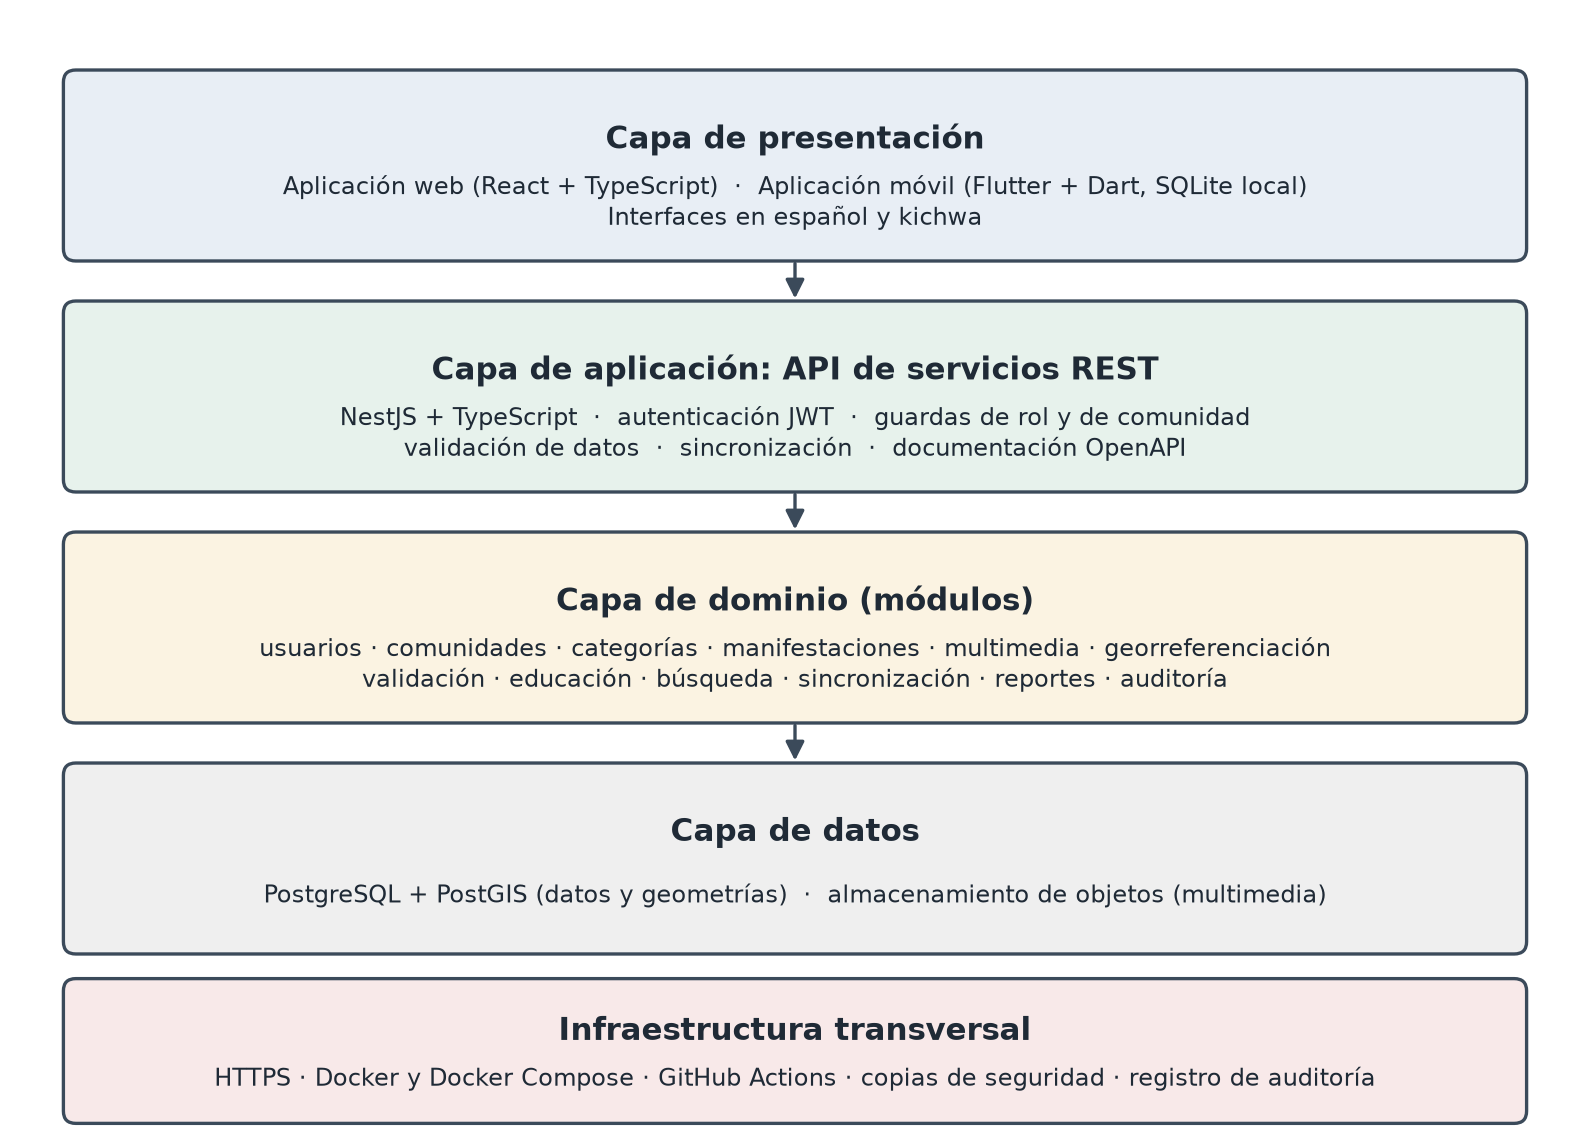
\includegraphics[width=0.85\textwidth]{Capítulos/img/arquitectura_capas.png}
  \caption{Arquitectura lógica por capas de la plataforma.}
  \label{img:arquitectura_capas}
\end{imagen}
\elaboradopor{Michael Jhosue Almeida Díaz}
\fuente{Elaboración propia}

La \textit{capa de presentación} contiene las dos aplicaciones cliente: la aplicación web, utilizada sobre todo para la administración, y la aplicación móvil, orientada a la consulta. La \textit{capa de aplicación} es la API de servicios REST, que recibe todas las solicitudes, verifica la identidad y los permisos del usuario y coordina las operaciones. La \textit{capa de dominio} reúne las reglas de negocio, organizadas en módulos según el estilo de monolito modular. La \textit{capa de datos} almacena la información estructurada y las geometrías en PostgreSQL con PostGIS, y los archivos multimedia en un almacenamiento de objetos. Por último, la \textit{infraestructura transversal} agrupa los servicios que afectan a todas las capas, como el cifrado de las comunicaciones, los contenedores, la integración continua y las copias de seguridad.

En cuanto al despliegue, todos los componentes del servidor se ejecutan en contenedores Docker coordinados con Docker Compose. Los clientes se conectan mediante HTTPS a un proxy inverso, que es el único punto de entrada al servidor y redirige las solicitudes a la API. La API es el único componente con acceso a la base de datos. Los archivos multimedia no se envían a través de la API, sino que se suben y descargan mediante direcciones firmadas de corta duración, que el servidor genera solo para los usuarios autorizados.

\subsection{Módulos del servidor}
La Tabla~\ref{tab:modulos} describe los módulos en que se organiza el servidor. Cada módulo encapsula sus datos y su lógica y expone sus operaciones al resto del sistema mediante servicios bien definidos.

\needspace{28\baselineskip}
{\centering\singlespacing
  \captionof{table}{Módulos del servidor.}
  \label{tab:modulos}
  \begin{tabular}{|p{0.22\textwidth}|p{0.66\textwidth}|}
    \hline
    \textbf{Módulo} & \textbf{Responsabilidad} \tabularnewline
    \hline
    \raggedright\hspace{0pt}\texttt{auth} & \raggedright\hspace{0pt}Inicio de sesión, emisión y renovación de tokens, guardas de rol y de comunidad \tabularnewline
    \hline
    \raggedright\hspace{0pt}\texttt{users} & \raggedright\hspace{0pt}Usuarios, roles y asociación a comunidades \tabularnewline
    \hline
    \raggedright\hspace{0pt}\texttt{communities} & \raggedright\hspace{0pt}Comunidades y su ubicación \tabularnewline
    \hline
    \raggedright\hspace{0pt}\texttt{categories} & \raggedright\hspace{0pt}Catálogo jerárquico de categorías culturales \tabularnewline
    \hline
    \raggedright\hspace{0pt}\texttt{manifestations} & \raggedright\hspace{0pt}Manifestaciones, traducciones, estados y niveles de acceso \tabularnewline
    \hline
    \raggedright\hspace{0pt}\texttt{media} & \raggedright\hspace{0pt}Carga, validación y optimización de archivos y generación de direcciones firmadas \tabularnewline
    \hline
    \raggedright\hspace{0pt}\texttt{geo} & \raggedright\hspace{0pt}Consultas espaciales y entrega de datos en formato GeoJSON \tabularnewline
    \hline
    \raggedright\hspace{0pt}\texttt{review} & \raggedright\hspace{0pt}Flujo de validación y observaciones \tabularnewline
    \hline
    \raggedright\hspace{0pt}\texttt{education} & \raggedright\hspace{0pt}Fichas informativas y cuestionarios \tabularnewline
    \hline
    \raggedright\hspace{0pt}\texttt{search} & \raggedright\hspace{0pt}Búsqueda de texto completo y filtros \tabularnewline
    \hline
    \raggedright\hspace{0pt}\texttt{sync} & \raggedright\hspace{0pt}Paquetes de descarga y cambios incrementales para la aplicación móvil \tabularnewline
    \hline
    \raggedright\hspace{0pt}\texttt{reports} & \raggedright\hspace{0pt}Indicadores del panel de administración \tabularnewline
    \hline
    \raggedright\hspace{0pt}\texttt{audit} & \raggedright\hspace{0pt}Registro de las acciones relevantes \tabularnewline
    \hline
  \end{tabular}\par}
\elaboradopor{Michael Jhosue Almeida Díaz}
\fuente{Elaboración propia}

\subsection{Modelo de datos}
El modelo de datos es relacional: la información se organiza en tablas relacionadas entre sí, en lugar de concentrarse en un único formulario. Esta decisión permite, por ejemplo, que una manifestación se vincule con varios lugares, categorías y recursos multimedia, y que cada recurso tenga su propio consentimiento. La Tabla~\ref{tab:entidades} describe las entidades principales.

\needspace{30\baselineskip}
{\centering\singlespacing
  \captionof{table}{Entidades principales del modelo de datos.}
  \label{tab:entidades}
  \begin{tabular}{|p{0.27\textwidth}|p{0.61\textwidth}|}
    \hline
    \textbf{Entidad} & \textbf{Descripción y campos principales} \tabularnewline
    \hline
    \raggedright\hspace{0pt}Usuario y rol & \raggedright\hspace{0pt}Persona registrada, con nombre, correo, contraseña cifrada y estado; puede tener uno o varios roles y pertenecer a comunidades \tabularnewline
    \hline
    \raggedright\hspace{0pt}Comunidad & \raggedright\hspace{0pt}Nombre, pueblo, provincia, cantón, parroquia, descripción y ubicación \tabularnewline
    \hline
    \raggedright\hspace{0pt}Lugar & \raggedright\hspace{0pt}Sitio asociado a una comunidad, con su geometría exacta, su geometría pública aproximada y la indicación de si es sensible \tabularnewline
    \hline
    \raggedright\hspace{0pt}Categoría & \raggedright\hspace{0pt}Clasificación cultural jerárquica con nombre en español y en kichwa \tabularnewline
    \hline
    \raggedright\hspace{0pt}Manifestación & \raggedright\hspace{0pt}Estado, nivel de acceso, autoría, fuente, fecha de registro, palabras clave, comunidad de origen y fecha de publicación \tabularnewline
    \hline
    \raggedright\hspace{0pt}Traducción & \raggedright\hspace{0pt}Título y descripción de una manifestación en un idioma, con la indicación de si está validada \tabularnewline
    \hline
    \raggedright\hspace{0pt}Recurso multimedia & \raggedright\hspace{0pt}Imagen, audio, video o documento, con su tipo de archivo, tamaño, duración, autoría y nivel de acceso \tabularnewline
    \hline
    \raggedright\hspace{0pt}Consentimiento & \raggedright\hspace{0pt}Persona que lo otorga, fecha, alcance y documento de respaldo de cada recurso \tabularnewline
    \hline
    \raggedright\hspace{0pt}Revisión & \raggedright\hspace{0pt}Decisión del revisor, observaciones y fecha \tabularnewline
    \hline
    \raggedright\hspace{0pt}Recurso educativo & \raggedright\hspace{0pt}Ficha o cuestionario vinculado a una manifestación, con sus preguntas \tabularnewline
    \hline
    \raggedright\hspace{0pt}Registro de auditoría & \raggedright\hspace{0pt}Usuario, acción, entidad afectada, datos del cambio y fecha \tabularnewline
    \hline
  \end{tabular}\par}
\elaboradopor{Michael Jhosue Almeida Díaz}
\fuente{Elaboración propia}

Las geometrías se almacenan en el sistema de referencia WGS84, identificado por el código SRID 4326, que es el que utiliza el formato GeoJSON \cite{butler2016geojson}. Para acelerar las consultas espaciales se crean índices espaciales sobre las geometrías, y para la búsqueda se crea un índice de texto completo sobre el título, la descripción y las palabras clave \cite{postgis2026docs}. Todas las tablas incluyen la fecha de su última actualización, que la sincronización móvil utiliza para identificar los cambios.

\subsection{Flujo de validación y niveles de acceso}
Cada manifestación atraviesa un ciclo de estados que garantiza que ningún contenido se publique sin la aprobación de la comunidad, tal como muestra la Imagen~\ref{img:flujo_validacion}. El investigador o el editor registra la manifestación en estado de borrador y la envía a revisión. El representante de la comunidad de origen la aprueba o la rechaza con observaciones, en cuyo caso vuelve a borrador. Solo el administrador puede publicar un contenido aprobado y, si fuera necesario, retirarlo. Además, una manifestación no puede publicarse si alguno de sus recursos multimedia carece de consentimiento registrado.

\begin{imagen}[htbp]
  \centering
  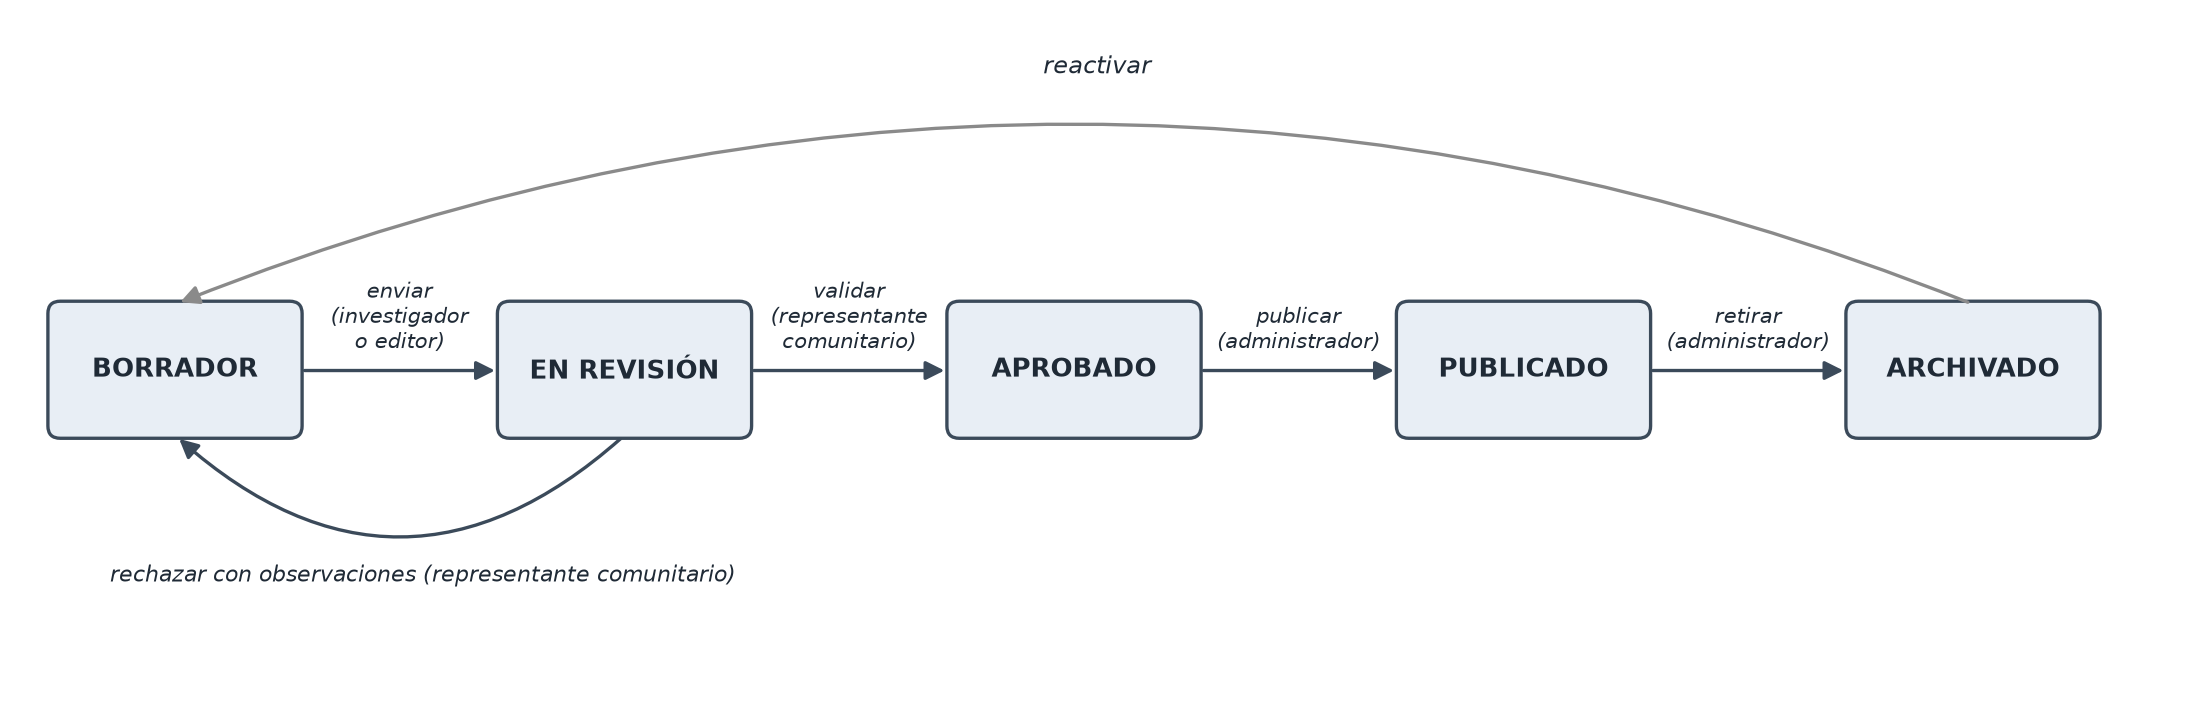
\includegraphics[width=0.95\textwidth]{Capítulos/img/flujo_validacion.png}
  \caption{Flujo de validación de las manifestaciones culturales.}
  \label{img:flujo_validacion}
\end{imagen}
\elaboradopor{Michael Jhosue Almeida Díaz}
\fuente{Elaboración propia}

De forma independiente al estado, cada manifestación y cada recurso tienen un nivel de acceso, descrito en la Tabla~\ref{tab:niveles_acceso}, que determina quién puede verlos.

\needspace{14\baselineskip}
{\centering\singlespacing
  \captionof{table}{Niveles de acceso a los contenidos.}
  \label{tab:niveles_acceso}
  \begin{tabular}{|p{0.18\textwidth}|p{0.40\textwidth}|p{0.30\textwidth}|}
    \hline
    \textbf{Nivel} & \textbf{Quién puede verlo} & \textbf{Descarga sin conexión} \tabularnewline
    \hline
    \raggedright\hspace{0pt}Público & \raggedright\hspace{0pt}Cualquier persona, incluido el visitante sin cuenta & \raggedright\hspace{0pt}Permitida \tabularnewline
    \hline
    \raggedright\hspace{0pt}Restringido & \raggedright\hspace{0pt}Usuarios autenticados con rol institucional & \raggedright\hspace{0pt}No permitida \tabularnewline
    \hline
    \raggedright\hspace{0pt}Reservado & \raggedright\hspace{0pt}Solo el administrador y los representantes de la comunidad de origen & \raggedright\hspace{0pt}No permitida; nunca se publica \tabularnewline
    \hline
  \end{tabular}\par}
\elaboradopor{Michael Jhosue Almeida Díaz}
\fuente{Elaboración propia}

En cuanto a la georreferenciación, cada lugar marcado como sensible conserva dos geometrías: la exacta, visible solo para los usuarios autorizados por la comunidad, y una pública de precisión reducida, por ejemplo redondeada a aproximadamente un kilómetro, que es la única que se envía al resto de usuarios. Esta regla se aplica en el servidor, de modo que la coordenada exacta nunca llega a un dispositivo no autorizado, y concreta la técnica de ofuscación descrita en la fundamentación teórica \cite{duckham2005obfuscation}.

\subsection{Funcionamiento sin conexión}
La aplicación móvil sigue un enfoque \textit{offline-first} de solo lectura \cite{kleppmann2019local}: siempre lee los contenidos desde su base de datos local SQLite y los actualiza en segundo plano cuando dispone de conexión. El usuario elige qué comunidades o categorías descargar y puede ver el espacio que ocupan. Solo se descargan contenidos públicos y publicados, es decir, fichas, textos, imágenes optimizadas, ubicaciones y recursos educativos; los videos se descargan únicamente si el usuario lo solicita.

Para la sincronización, la aplicación guarda la fecha de su última actualización y solicita a la API solo los contenidos creados, modificados o retirados desde entonces. Como la aplicación móvil no edita contenidos, no pueden producirse conflictos entre versiones, y la versión del servidor prevalece siempre. Si un contenido deja de ser público, la sincronización lo elimina del dispositivo.

\subsection{Interfaces de usuario}
Las interfaces se diseñarán primero como prototipos en Figma y se validarán con usuarios representativos antes de programarlas. Ambas aplicaciones incluirán un selector de idioma entre español y kichwa; si un contenido no tiene traducción validada al kichwa, se mostrará en español. Los elementos gráficos con referencias culturales se validarán con los representantes comunitarios, para evitar el uso de símbolos como simple decoración descontextualizada.

La aplicación web incluirá las pantallas de inicio de sesión, panel de indicadores, comunidades, categorías, manifestaciones, multimedia, mapa, cola de revisión, recursos educativos, usuarios y reportes. La aplicación móvil incluirá las pantallas de inicio, exploración por categoría, mapa, buscador, ficha de manifestación con reproductor multimedia, recursos educativos y cuestionarios, descargas sin conexión, favoritos y ajustes de idioma.

\section{Justificación Técnica}
La selección de las tecnologías se basó en cinco criterios derivados de los requerimientos: la capacidad de cubrir las plataformas objetivo con un equipo de una sola persona, el soporte para datos geográficos, el funcionamiento sin conexión, la mantenibilidad del código y el uso de herramientas de código abierto sin costos de licencia. Las Tablas~\ref{tab:justificacion} y~\ref{tab:justificacion2} resumen las principales decisiones, las alternativas consideradas y el motivo de la elección.

\needspace{30\baselineskip}
{\centering\singlespacing
  \captionof{table}{Justificación de las decisiones tecnológicas.}
  \label{tab:justificacion}
  \begin{tabular}{|p{0.16\textwidth}|p{0.20\textwidth}|p{0.16\textwidth}|p{0.33\textwidth}|}
    \hline
    \textbf{Decisión} & \textbf{Alternativas consideradas} & \textbf{Elección} & \textbf{Motivo} \tabularnewline
    \hline
    \raggedright\hspace{0pt}Aplicación móvil & \raggedright\hspace{0pt}Desarrollo nativo por plataforma; otros marcos multiplataforma & \raggedright\hspace{0pt}Flutter & \raggedright\hspace{0pt}Una sola base de código para Android e iOS con compilación a código nativo \cite{flutter2026docs} \tabularnewline
    \hline
    \raggedright\hspace{0pt}Aplicación web & \raggedright\hspace{0pt}Next.js; otras bibliotecas de interfaz & \raggedright\hspace{0pt}React con TypeScript & \raggedright\hspace{0pt}Componentes reutilizables para formularios y tablas \cite{react2026docs}; el panel no requiere renderizado en servidor \tabularnewline
    \hline
    \raggedright\hspace{0pt}Servidor & \raggedright\hspace{0pt}FastAPI (Python); NestJS & \raggedright\hspace{0pt}NestJS & \raggedright\hspace{0pt}Mismo lenguaje, TypeScript, que la aplicación web; organización en módulos y guardas de acceso \cite{nestjs2026docs} \tabularnewline
    \hline
    \raggedright\hspace{0pt}Estilo del servidor & \raggedright\hspace{0pt}Microservicios; monolito modular & \raggedright\hspace{0pt}Monolito modular & \raggedright\hspace{0pt}Menor complejidad de despliegue para un equipo pequeño, con separación por dominio \cite{richards2020fundamentals} \tabularnewline
    \hline
    \raggedright\hspace{0pt}Base de datos & \raggedright\hspace{0pt}Base de datos de documentos en la nube, como la del prototipo previo; PostgreSQL & \raggedright\hspace{0pt}PostgreSQL con PostGIS & \raggedright\hspace{0pt}Integridad relacional entre manifestaciones, lugares y consentimientos, y consultas espaciales nativas \cite{postgis2026docs} \tabularnewline
    \hline
      \end{tabular}\par}
\elaboradopor{Michael Jhosue Almeida Díaz}
\fuente{Elaboración propia}

\needspace{18\baselineskip}
{\centering\singlespacing
  \captionof{table}{Justificación de las decisiones tecnológicas (continuación).}
  \label{tab:justificacion2}
  \begin{tabular}{|p{0.16\textwidth}|p{0.20\textwidth}|p{0.16\textwidth}|p{0.33\textwidth}|}
    \hline
    \textbf{Decisión} & \textbf{Alternativas consideradas} & \textbf{Elección} & \textbf{Motivo} \tabularnewline
    \hline
    \raggedright\hspace{0pt}Mapas & \raggedright\hspace{0pt}Kits de mapas comerciales; Leaflet; MapLibre & \raggedright\hspace{0pt}MapLibre & \raggedright\hspace{0pt}Código abierto, mapas vectoriales y disponibilidad para web y móvil \cite{maplibre2026docs} \tabularnewline
    \hline
    \raggedright\hspace{0pt}Almacenamiento local & \raggedright\hspace{0pt}Archivos sueltos; SQLite & \raggedright\hspace{0pt}SQLite & \raggedright\hspace{0pt}Consultas estructuradas en el dispositivo para el funcionamiento sin conexión \tabularnewline
    \hline
    \raggedright\hspace{0pt}Despliegue & \raggedright\hspace{0pt}Instalación manual; contenedores & \raggedright\hspace{0pt}Docker y Docker Compose & \raggedright\hspace{0pt}Entornos reproducibles e instalación documentada en cualquier servidor \tabularnewline
    \hline
  \end{tabular}\par}
\elaboradopor{Michael Jhosue Almeida Díaz}
\fuente{Elaboración propia}

La decisión más relevante es la de la base de datos. El prototipo Saraguro utilizaba servicios de Firebase \cite{quezada2026mobile}, adecuados para una aplicación de consulta, pero el nuevo alcance exige relacionar de forma rigurosa manifestaciones, comunidades, lugares, recursos, consentimientos, revisiones y registros de auditoría, y garantizar que ninguna regla de integridad se incumpla; por ejemplo, que no exista un recurso publicado sin consentimiento. Una base de datos relacional asegura estas reglas en el propio motor, y la extensión PostGIS añade las consultas espaciales que requiere el módulo de georreferenciación \cite{postgis2026docs}.

Del mismo modo, la elección de Flutter responde a la restricción de recursos humanos: con un solo desarrollador, mantener dos aplicaciones nativas independientes no sería viable dentro del plazo del proyecto, mientras que una base de código única permite dedicar ese esfuerzo a las funciones que aportan valor, como la consulta sin conexión y la protección de los contenidos \cite{flutter2026docs,biorn2019cross}.

Finalmente, algunas decisiones técnicas permanecen abiertas porque dependen de condiciones institucionales o de la participación de las comunidades. Se resolverán durante los sprints indicados en la Tabla~\ref{tab:decisiones_abiertas}.

\needspace{20\baselineskip}
{\centering\singlespacing
  \captionof{table}{Decisiones técnicas abiertas.}
  \label{tab:decisiones_abiertas}
  \begin{tabular}{|p{0.25\textwidth}|p{0.40\textwidth}|p{0.23\textwidth}|}
    \hline
    \textbf{Decisión} & \textbf{Opciones} & \textbf{Responsable} \tabularnewline
    \hline
    \raggedright\hspace{0pt}Almacenamiento multimedia & \raggedright\hspace{0pt}Almacenamiento institucional compatible con S3 o Firebase Storage & \raggedright\hspace{0pt}Autor y CICHE \tabularnewline
    \hline
    \raggedright\hspace{0pt}Alojamiento & \raggedright\hspace{0pt}Servidor institucional o servicio en la nube & \raggedright\hspace{0pt}CICHE \tabularnewline
    \hline
    \raggedright\hspace{0pt}Mapas sin conexión & \raggedright\hspace{0pt}Teselas descargables por región o solo marcadores sin mapa base & \raggedright\hspace{0pt}Autor \tabularnewline
    \hline
    \raggedright\hspace{0pt}Proveedor de teselas & \raggedright\hspace{0pt}OpenStreetMap, servicio comercial o servidor propio & \raggedright\hspace{0pt}Autor \tabularnewline
    \hline
    \raggedright\hspace{0pt}Muestra inicial de contenidos & \raggedright\hspace{0pt}Comunidades y manifestaciones según el proyecto Kallarimanta & \raggedright\hspace{0pt}Tutor y comunidades \tabularnewline
    \hline
    \raggedright\hspace{0pt}Validación lingüística en kichwa & \raggedright\hspace{0pt}Especialista asignado & \raggedright\hspace{0pt}CICHE \tabularnewline
    \hline
    \raggedright\hspace{0pt}Publicación en tiendas de aplicaciones & \raggedright\hspace{0pt}Publicar o distribuir solo el instalador de pruebas & \raggedright\hspace{0pt}Tutor \tabularnewline
    \hline
  \end{tabular}\par}
\elaboradopor{Michael Jhosue Almeida Díaz}
\fuente{Elaboración propia}
